%document
\documentclass[10pt]{beamer}
%theme
\usetheme{metropolis}
% packages
\usepackage{color}
\usepackage{listings}
\usepackage[ngerman]{babel}
\usepackage[utf8]{inputenc}
\usepackage{multicol}

\usepackage{hyperref}
\hypersetup{colorlinks=true, linkcolor=blue, urlcolor=red}

% color definitions
\definecolor{mygreen}{rgb}{0,0.6,0}
\definecolor{mygray}{rgb}{0.5,0.5,0.5}
\definecolor{mymauve}{rgb}{0.58,0,0.82}

\lstset{
    backgroundcolor=\color{white},
    % choose the background color;
    % you must add \usepackage{color} or \usepackage{xcolor}
    basicstyle=\footnotesize\ttfamily,
    % the size of the fonts that are used for the code
    breakatwhitespace=false,
    % sets if automatic breaks should only happen at whitespace
    breaklines=true,                 % sets automatic line breaking
    captionpos=b,                    % sets the caption-position to bottom
    commentstyle=\color{mygreen},    % comment style
    % deletekeywords={...},
    % if you want to delete keywords from the given language
    extendedchars=true,
    % lets you use non-ASCII characters;
    % for 8-bits encodings only, does not work with UTF-8
    frame=single,                    % adds a frame around the code
    keepspaces=true,
    % keeps spaces in text,
    % useful for keeping indentation of code
    % (possibly needs columns=flexible)
    keywordstyle=\color{blue},       % keyword style
    % morekeywords={*,...},
    % if you want to add more keywords to the set
    numbers=left,
    % where to put the line-numbers; possible values are (none, left, right)
    numbersep=5pt,
    % how far the line-numbers are from the code
    numberstyle=\tiny\color{mygray},
    % the style that is used for the line-numbers
    rulecolor=\color{black},
    % if not set, the frame-color may be changed on line-breaks
    % within not-black text (e.g. comments (green here))
    stepnumber=1,
    % the step between two line-numbers.
    % If it's 1, each line will be numbered
    stringstyle=\color{mymauve},     % string literal style
    tabsize=4,                       % sets default tabsize to 4 spaces
    % show the filename of files included with \lstinputlisting;
    % also try caption instead of title
    language = C,
	showspaces = false,
	showtabs = false,
	showstringspaces = false,
	escapechar = ,
}

\def\ContinueLineNumber{\lstset{firstnumber=last}}
\def\StartLineAt#1{\lstset{firstnumber=#1}}
\let\numberLineAt\StartLineAt



\newcommand{\codeline}[1]{
	\alert{\texttt{#1}}
}

% This Document contains the information about this course.

% Authors of the slides
\author{
    Lecturers:
	%name1
	Mirko Jantschke,
	%name2
	Pascal Scholz
	\\
	%creaters of the slides
	Created by: Richard Mörbitz, Manuel Thieme
}


% Fancy Logo
\titlegraphic{\hfill
\includegraphics[height=1.25cm]{../templates/fsr_logo_cropped}}


\title{C-Lessons}
\subtitle{Pointers and Memory}
\date{\today}

\usetikzlibrary{tikzmark}
\usetikzlibrary{arrows}
\tikzset{arrow/.style={-latex, shorten >=.5ex, shorten <=.5ex}}
\lstset{
  moredelim=**[is][\only<+(1)>{\color{red}}]{§}{§},
}

% the actual document
\begin{document}

\maketitle

\begin{frame}{Contents}
	\tableofcontents
\end{frame}

%---------------------------------------------------------------------------------------------------------------------------
\section{Pointers}
%---------------------------------------------------------------------------------------------------------------------------

\begin{frame}[fragile]{RGB}
	Consider a function that calculates the RGB values of a hex color string:
	\begin{lstlisting}[numbers=none]
int calcRGB(char hexString[]) {
	... 		/* converting hexString into RGB values */
	return ???;
}
\end{lstlisting}
	\begin{itemize}
		\item It is not possible to return 3 values.
	\end{itemize}
	We could write 3 different functions:
	\begin{lstlisting}[numbers=none]
int calcR(char hexString[]) { ... }	/* returns R value */
int calcG(char hexString[]) { ... }	/* returns G value */
int calcB(char hexString[]) { ... }	/* returns B value */
\end{lstlisting}
	Or we declare the 3 variables before the function call and just tell the function were to put the values.
\end{frame}

%---------------------------------------------------------------------------------------------------------------------------

\begin{frame}{Memory again}
	\begin{itemize}[<+->]
		\item You have two int variables in your main function.
		\item Now you call a function
		\item You want to change the value of a variable in the main scope
	\end{itemize}
	\begin{textblock}{10}(1,6.5)
		\begin{tikzpicture}[font=\scriptsize,x=2.5cm]
			
			\draw (0,1) -- (4,1);
			\draw (0,1) -- (0,1.3);
			\draw (0,1.3) -- (4,1.3);
			\draw (4,1) -- (4,1.3);
			
			\node[above=.6em] at (0,1) {\#0};
			\draw[dashed] (.5,1) -- (.5,1.3);
			\node[above=.6em] at (.5,1) {\#4};
			\draw[dashed] (1,1) -- (1,1.3);
			\node[above=.6em] at (1,1) {\#8};
			\draw[dashed] (1.5,1) -- (1.5,1.3);
			\node[above=.6em] at (1.5,1) {\#12};
			\draw[dashed] (2,1) -- (2,1.3);
			\node[above=.6em] at (2,1) {\#16};
			\draw[dashed] (2.5,1) -- (2.5,1.3);
			\node[above=.6em] at (2.5,1) {\#20};
			\draw[dashed] (3,1) -- (3,1.3);
			\node[above=.6em] at (3,1) {\#24};
			\draw[dashed] (3.5,1) -- (3.5,1.3);
			\node[above=.6em] at (3.5,1) {\#28};
			
			\node[blue, below=.4em, right=0em] at (0.15,1.3) {int};
			\draw[dashed, blue] (0,1) -- (.5,1);
			\draw[dashed, blue] (.5,1) -- (.5,1.3);
			\draw[dashed, blue] (0,1.3) -- (.5,1.3);
			\draw[dashed, blue] (0,1) -- (0,1.3);
		
			\node[blue, below=.4em, right=0em] at (.65,1.3) {int};
			\draw[dashed, blue] (.5,1) -- (1,1);
			\draw[dashed, blue] (1,1) -- (1,1.3);
			\draw[dashed, blue] (.5,1.3) -- (1,1.3);
			\draw[dashed, blue] (.5,1) -- (.5,1.3);
			
			
			\draw[orange, dashed] (-.2,.6) -- (-.2,1.9) node[right=1.7em, above=0em]{Main scope};
			\draw[orange, dashed] (-.2,.6) -- (1,.6);
			\draw[orange, dashed] (1,.6) -- (1,1.9);
			\draw[orange, dashed] (-.2,1.9) -- (1,1.9);		
			
			\begin{uncoverenv}<5->
				\node[teal, below=.4em, right=0em] at (1.4,1.3) {int*};
				\draw[dashed, teal] (1,1) -- (2,1);
				\draw[dashed, teal] (2,1) -- (2,1.3);
				\draw[dashed, teal] (1,1.3) -- (2,1.3);
				\draw[dashed, teal] (1,1) -- (1,1.3);
				\draw (1.5,1) edge[teal,out=220,in=0,shorten >=0ex,shorten <=.5ex] (1.2,.7);
			\end{uncoverenv}		
			
			\begin{uncoverenv}<6->
				\node[teal, below=.4em, right=0em] at (2.4,1.3) {int*};
				\draw[dashed, teal] (2,1) -- (3,1);
				\draw[dashed, teal] (3,1) -- (3,1.3);
				\draw[dashed, teal] (2,1.3) -- (3,1.3);
				\draw[dashed, teal] (2,1) -- (2,1.3);
			
				\node[teal, below=.4em, right=0em] at (3.4,1.3) {int*};
				\draw[dashed, teal] (3,1) -- (4,1);
				\draw[dashed, teal] (4,1) -- (4,1.3);
				\draw[dashed, teal] (3,1.3) -- (4,1.3);
				\draw[dashed, teal] (3,1) -- (3,1.3);
			\end{uncoverenv}		
			
			\begin{uncoverenv}<6->
				\draw[arrow, teal, bend angle=45, bend left] (2.5,1) to (.25,1);
				\draw[arrow, teal, bend angle=50, bend left] (3.5,1) to (.25,1);
			\end{uncoverenv}		
			
			\begin{uncoverenv}<6->
				\draw (.15,.9) -- (.15,.6) node[below]{\textit{int a;}};
				\draw (.75,.9) -- (.75,.6) node[below]{\textit{int b;}};
				\draw (1.5,.9) -- (1.5,.6) node[below]{\textit{int* pb = \&b;}};
				\draw (2.6,.9) -- (2.6,.6) node[below]{\textit{int* pa = \&a;}};
				\draw (3.8,.9) -- (3.8,.6) node[below]{\textit{int* ndpa = \&a;}};
			\end{uncoverenv}
			
			\begin{uncoverenv}<2->
				\draw[red, dashed] (1,.6) -- (1,1.9) node[right=2.3em, above=0em]{Function scope};
				\draw[red, dashed] (1,.6) -- (4.2,.6);
				\draw[red, dashed] (4.2,.6) -- (4.2,1.9);
				\draw[red, dashed] (1,1.9) -- (4.2,1.9);
			\end{uncoverenv}
			
			\draw<3-> (1.2,.7) edge[teal,out=180,in=320,arrow,shorten >=.5ex,shorten <=0ex] (.75,1);
		\end{tikzpicture}
	\end{textblock}
	\ \\\ \\\ \\\ \\\ \\\ \\\ \\\ \\\ \\
	\begin{itemize}[<+->]
		\item You'll have to pass the address of this variable
		\item This address is stored in a \textit{pointer} variable
		\item This method is called \textit{call by reference}
	\end{itemize}
\end{frame}

%---------------------------------------------------------------------------------------------------------------------------

\begin{frame}[fragile]{Operators}
	\begin{itemize}
		\item To declare a Pointer, use the \textit{dereference operator} \textbf{*}
		\item To get the address of a variable, C offers the \textit{address operator} \textbf{\&}
		\item To access the variable a pointer points to, dereference it with the \textit{dereference operator} \textbf{*}
	\end{itemize}
	\begin{lstlisting}[numbers=none]
int a = 42;
int *pa;	/* declare an int pointer*/
pa = &a;	/* initialize pa as pointer to a */
*pa = 13;	/* change a */
    \end{lstlisting}
\end{frame}

%---------------------------------------------------------------------------------------------------------------------------

\begin{frame}[fragile]{Increment and decrement}
	If you want to increment or decrement the variable a pointer points to, you have to use Parentheses.
	\begin{lstlisting}[numbers=none]
int a = 42;
int *pa = &a;	/* define pa as pointer to a */
(*pa)++;		/* increment a */
(*pa)--;		/* decrement a */
\end{lstlisting}
\ \\\ \\
If you had not used the parentheses, you would have in-/decremented the pointer, not the variable it points to. 
Congratulations, you just invented pointer arithmetic but we will talk later about that.
\end{frame}

%---------------------------------------------------------------------------------------------------------------------------

\begin{frame}[fragile]{Back to RGB}
	Now we can think of the RGB function as one function, taking the hexString and 3 Pointers:
	\begin{lstlisting}[numbers=none]
void calcRGB(char hexString[], int *r, int *g, int *b) {
	...
	*r = calculatedRValue;
	*g = calculatedGValue;
	*b = calculatedBValue;
}
\end{lstlisting}
	Call it with
	\begin{lstlisting}[numbers=none]
int r, g, b;
calcRGB("ffffff", &r, &g, &b);
\end{lstlisting}
	\begin{itemize}
		\item You now should understand how scanf works.
	\end{itemize}
\end{frame}

%---------------------------------------------------------------------------------------------------------------------------

\begin{frame}[fragile]{Returning pointers}
Pointers can be return values, too.\\\ \\
\textbf{But} 
	\begin{lstlisting}[numbers=none]
int *someFunction(void) {	
	int a = 42;
	return &a;
}
\end{lstlisting}
	\begin{itemize}
		\item Dafuq did just happen?
	\end{itemize}
\end{frame}

%---------------------------------------------------------------------------------------------------------------------------
\section{Pointer arithmetic}
%---------------------------------------------------------------------------------------------------------------------------

\begin{frame}[fragile]{p++}
	You can in-/decrement a pointer. If you do so, the address it points to will change.\\
	The address changes by the size of the pointer type.
	\begin{columns}[T]
		\column{.5\textwidth}
		\begin{lstlisting}[numbers=none]
int a, b;
long c;
int *p = &a;
p++;
p++;
p++;
\end{lstlisting}
		\column{.5\textwidth}
		\begin{tikzpicture}[font=\scriptsize,x=2.5cm]
				
			\draw (0,1) -- (2,1);
			\draw (0,1) -- (0,1.3);
			\draw (0,1.3) -- (2,1.3);
			\draw (2,1) -- (2,1.3);
			
			\node[above=.6em] at (0,1) {\#0};
			\draw[dashed] (.5,1) -- (.5,1.3);
			\node[above=.6em] at (.5,1) {\#4};
			\draw[dashed] (1,1) -- (1,1.3);
			\node[above=.6em] at (1,1) {\#8};
			\draw[dashed] (1.5,1) -- (1.5,1.3);
			\node[above=.6em] at (1.5,1) {\#12};
			\draw[dashed] (2,1) -- (2,1.3);
			
			\node[blue, below=-.15em] at (0.25,1.3) {int a};
			\node[blue, below=-.15em] at (.75,1.3) {int b};
			\node[teal, below=-.15em] at (1.5,1.3) {long c};
			\begin{uncoverenv}<2>
				\draw (2.1,1.2) edge[teal,out=225,in=315,arrow,shorten >=.5ex,shorten <=.5ex] (0,1);
			\end{uncoverenv}
			\begin{uncoverenv}<3>
				\draw (2.1,1.2) edge[teal,out=225,in=315,arrow,shorten >=.5ex,shorten <=.5ex] (.5,1);
			\end{uncoverenv}
			\begin{uncoverenv}<4>
				\draw (2.1,1.2) edge[teal,out=225,in=315,arrow,shorten >=.5ex,shorten <=.5ex] (1,1);
			\end{uncoverenv}
			\begin{uncoverenv}<5>
				\draw (2.1,1.2) edge[teal,out=225,in=315,arrow,shorten >=.5ex,shorten <=.5ex] (1.5,1);
			\end{uncoverenv}
		\end{tikzpicture}
	\end{columns}
	\begin{itemize}
		\item<5-> Since the pointer is of type \textit{int *}, the target address moves only the size of \textit{int}
	\end{itemize}
\end{frame}

%---------------------------------------------------------------------------------------------------------------------------

\begin{frame}[fragile]{Pointers and arrays}
	The identifier of an array can be considered a pointer.\\
	This means we can consider the index as an offset for the pointer and access array elements trough pointer arithmetic:
	\begin{lstlisting}[numbers=none]
int leet[4] = {1, 3, 3, 7};
int *pleet = leet;
*(pleet++) = 2;
printf("%d %d\n", *pleet, *(pleet + 2));
\end{lstlisting}
	\begin{itemize}
		\item What is the output?
	\end{itemize}
	\begin{uncoverenv}<2->
		\begin{lstlisting}[numbers=none]
3 7
\end{lstlisting}
		\begin{itemize}
			\item Why?
			\begin{itemize}
				\item<3-> Hint: Wasn't there a difference between \textit{c++} and \textit{++c} ?
			\end{itemize}
		\end{itemize}
	\end{uncoverenv}
\end{frame}

%---------------------------------------------------------------------------------------------------------------------------
\section{Features of pointers}
%---------------------------------------------------------------------------------------------------------------------------

\begin{frame}[fragile]{\textbf{argc} and \textbf{argv}}
	You can pass strings to your program from the command line:
	\begin{lstlisting}[numbers=none]
./a.out string1 longer_string2
\end{lstlisting}
	\bigskip
	You will have to use an alternative definition of \textit{main()}:
	\begin{lstlisting}[numbers=none]
int main(int argc, char *argv[]) {
\end{lstlisting}
	\begin{itemize}
		\item The arguments are stored in \textit{argv}\footnote{Short for \textit{argument value}}
		\item \textit{argv} is an array of pointers to the first character of a string
		\item \textbf{Caution:} \textit{argv[0]} is the name by which you called the program
		\item \textit{argc}\footnote{Short for \textit{argument count}} is the number of strings stored in \textit{argv}
	\end{itemize}
\end{frame}

%---------------------------------------------------------------------------------------------------------------------------

\begin{frame}[fragile]{Misc.}
	As pointers hold addresses, print them as positive hexadecimal numbers!\\
	\textit{Printf()} has a special placeholder \textbf{\%p} for that.\\
	\begin{lstlisting}[numbers=none]
int a;	/* assume address 42 */
int *b = &a;
printf("%p\n", b);	/* output: 0x2a */
\end{lstlisting}
	\pause
	\bigskip
	Caution: the \textbf{*} operator always refers to the next identifier:
	\begin{lstlisting}[numbers=none]
int *a, *b;	/* two pointers */
int* a, b;	/* pointer and int */
\end{lstlisting}
	\bigskip
	Some people prefer \textit{int* a} over \textit{int *a}. This is fine, but avoid declarations as the one above. \only<3->{And keep it consistent.}
\end{frame}

%---------------------------------------------------------------------------------------------------------------------------

\begin{frame}{Segmentation Fault}
	\centerline{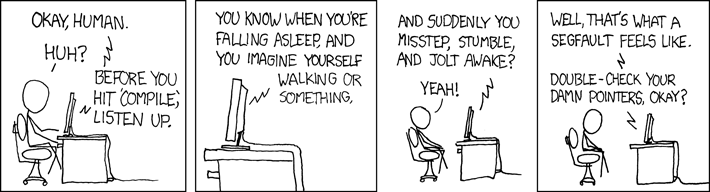
\includegraphics[scale=.4]{../img/compiler_complaint.png}
		\let\thefootnote\relax\footnote{\tiny "Compiler Complaint" by Randall Munroe. Licensed under \textit{Creative Commons Attribution-NonCommercial 2.5 License}}} \ \\[.5cm]
	A segmentation fault is very common when working with pointers.\\
	It means you were trying to write on memory your program didn't own. \\
	Try to avoid those errors, backtracing is hard!
\end{frame}

%-------------------------------------------------------------------------------------------------
\section{Related Task}
%-------------------------------------------------------------------------------------------------

\begin{frame}{Swap}
    \href{http://fsr.github.io/c-lessons/exercises/23_swap.html}{Task as online}
    \newline
    Write a function that swaps the values of 2 variables.
    \newline 
    \newline
    Experts: Write a function, that rotates 3 values in a given direction.
\end{frame}

%---------------------------------------------------------------------------------------------------------------------------

% TODO from here on: build your own content


\end{document}
